\documentclass[dvipsnames]{beamer}

\usepackage{amssymb,amsmath}
\usepackage{fixltx2e} % provides \textsubscript
\usepackage{mathspec}
\defaultfontfeatures{Ligatures=TeX, Scale=MatchLowercase}
\setmonofont[Scale=0.75]{Inconsolata}
\usetheme{metropolis}
% use microtype if available
\IfFileExists{microtype.sty}{%
\usepackage{microtype}
\UseMicrotypeSet[protrusion]{basicmath} % disable protrusion for tt fonts
}{}

\usepackage{polyglossia}
\setmainlanguage[]{french}
\usepackage{color}
\usepackage{pgfplots}
\pgfplotsset{compat=1.16}

% Prevent slide breaks in the middle of a paragraph:
\widowpenalties 1 10000
\raggedbottom

\setlength{\emergencystretch}{3em}  % prevent overfull lines
\providecommand{\tightlist}{%
  \setlength{\itemsep}{0pt}\setlength{\parskip}{0pt}}
\setcounter{secnumdepth}{0}
\PassOptionsToPackage{usenames,dvipsnames}{xcolor}

\usetikzlibrary{shapes, shapes.misc}
\definecolor{mDarkGreen}{HTML}{239541}

\usepackage{xpatch}
\xapptocmd\ttfamily{\XeTeXinterchartokenstate=0 }{}{}
\usepackage{minted}
\usemintedstyle{trac}

\usepackage[scale=2]{ccicons}
\usepackage{marvosym}
\usepackage{fourier-orns}
\usetikzlibrary{arrows}
\usetikzlibrary{calc}

\title{Une introduction à Python}
\subtitle{voire un peu plus\dots}
\author{Xavier Olive, ONERA}
\date{version 0.9999}
\institute{\ccbysa}

\def\interlude{
\begin{frame}[standout]
Interlude\\[1em]
    \centerline{\decothreeleft\;\rotatebox[origin=c]{180}{\decothreeleft}}
\end{frame}
}

\begin{document}
\frame{\titlepage}

\begin{frame}{Carte d'identité}

    Python est un langage de programmation:

    \begin{itemize}
        \tightlist
        \item interprété;
        \item multi-paradigme;
        \item multi-plateforme;
    \end{itemize}

    utilisé par une communauté importante:

    \begin{itemize}
        \tightlist
        \item une syntaxe simple;
        \item de nombreuses extensions;
        \item libre et gratuit.
    \end{itemize}

    \tikz[overlay, remember picture] \node[anchor=north east] at
    ($(current page.north east) + (-1,-2.5)$)
    {
        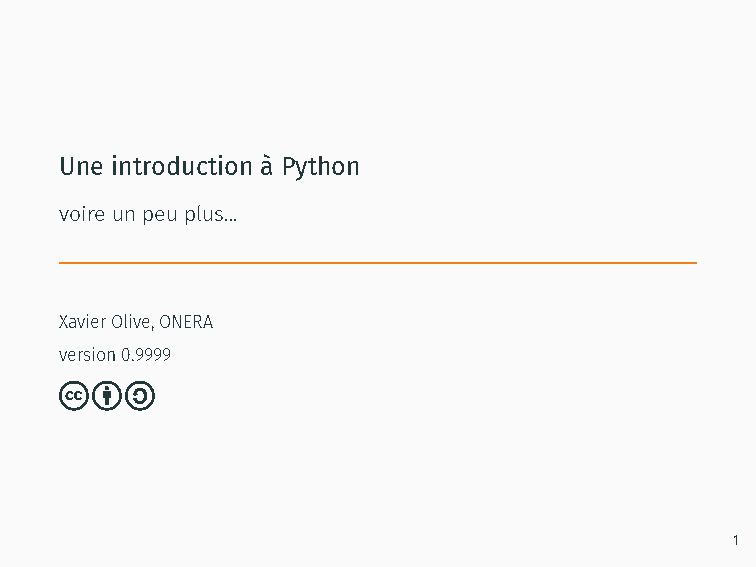
\includegraphics[width=1.5cm]{logo/python.png}
    };
\end{frame}

\begin{frame}
    [fragile]{Historique}
    \begin{tikzpicture}[>=stealth']
        \footnotesize
        \draw[->, semithick] (0, 0) -- (11, 0); % 0 -> 1990, 11 -> 2017, 0.25 = 1yr
        \draw (.4, 0.15) node[above] (py09) {1991} -- (.4, -0.15);
        \node[above of=py09, xshift=1em] (start) {Python 0.9};
        \node[below left of=start, node distance=2em, anchor=west] {\em
            \scriptsize Guido van Rossum, BDFL\footnote{BDFL: Benevolent Dictator For
                Life} $\longrightarrow$ 2018};
        \draw (7.2, 0.15) node[above] (py30) {2008} -- (7.2, -0.15);
        \node[above of=py30, xshift=-2em, text width=6em] (py2630) {Python
            2.6 Python 3.0};
        \draw (8, 0.15) node[above] (py27) {2010} -- (8, -0.15);
        \node[above of=py27, yshift=.7em] (py27-) {Python 2.7};
        \draw (9.5, 0.15) node[above] (py37) {'18} -- (9.5, -0.15);
        \draw (10, 0.15) node[above] (py38) {'19} -- (10, -0.15);
        \draw (10.5, 0.15) node[above] (py39) {'20} -- (10.5, -0.15);
        \node[above of=py37, yshift=-.7em] (py37-) {py37};
        \node[above of=py38, yshift=.3em] (py38-) {py38};
        \node[above of=py39, yshift=1.3em] (py39-) {py39};

        \draw[dashed] (py2630) -- (py30);
        \draw[dashed] (py27-) -- (py27);
        \draw[dashed] (py37-) -- (py37);

        \draw (2, 0.15) node[above] (95) {1995} -- (2, -0.15);
        \draw (4.4, 0.15) node[above] (01) {2001} -- (4.4, -0.15);
        \draw (6.4, 0.15) node[above] (06) {2006} -- (6.4, -0.15);

        \node [above of=01, yshift=2.5em, draw, semithick, inner sep=1ex] (psf)
        {PSF\footnote{PSF: Python Software Fundation}};
        \draw[dashed] (psf) -- (01);

        \fill[mLightBrown] (2, -.7) node[above, anchor=south west] {\scriptsize
            Numeric} rectangle (6.4, -.75);
        \fill[mLightBrown] (6.4, -.8) node[above, anchor=south west] {\scriptsize
            NumPy \em \tiny --- T. Oliphant (Anaconda)} rectangle (10.5, -.85);

        \fill[mLightBrown] (4.4, -1.4) node[above, anchor=south west] {\scriptsize
            Matplotlib \em \tiny --- J.D. Hunter \textdagger} rectangle (10.5, -1.45);

        \fill[mDarkGreen] (4.4, -2) node[above, anchor=south west] {\scriptsize
            Pyrex} rectangle (6.8, -2.05);
        \fill[mDarkGreen] (6.8, -2.1) node[above, anchor=south west] {\scriptsize
            Cython \em \tiny --- R. Bradshaw, S. Behnel} rectangle (10.5, -2.15);

        \fill[mDarkTeal] (4.4, -2.7) node[above, anchor=south west] {\scriptsize
            IPython \em \tiny --- F. Perez} rectangle (10.5, -2.75);
        \fill[mDarkTeal] (9.6, -3.3) node[above, anchor=south west] {\scriptsize
            Jupyter} rectangle (10.5, -3.35);

    \end{tikzpicture}

\end{frame}

\begin{frame}[fragile]{L'écosystème moderne}
\begin{tikzpicture}[>=stealth']
    \footnotesize
    % 2020-2025 timeline with new tools

    % Add PEP 518 note
    \draw[->, semithick] (0, 0) -- (10, 0); % extend to 2024
    \draw[->, semithick] (0, 0) -- (10, 0); % 0 -> 2020, 11 -> 2024, 1 = 1yr

    \draw (0, 0.15) node[above] (pep518) {'16} --  (0, -0.15);
    \draw (2, 0.15) node[above] (py37) {'18} --  (2, -0.15);
    \draw (3, 0.15) node[above] (py38) {'19} --  (3, -0.15);
    \draw (4, 0.15) node[above] (py39) {'20} --  (4, -0.15);
    \draw (5, 0.15) node[above] (py310) {'21} -- (5, -0.15);
    \draw (6, 0.15) node[above] (py311) {'22} -- (6, -0.15);
    \draw (7, 0.15) node[above] (py312) {'23} -- (7, -0.15);
    \draw (8, 0.15) node[above] (py313) {'24} -- (8, -0.15);
    \draw (9, 0.15) node[above] (py314) {'25} -- (9, -0.15);

    \node[above of=pep518, yshift=-.7em] (pep518-) {PEP518};
    \node[below of=pep518-, yshift=-3em] {\scriptsize pyproject.toml};
    \node[above of=py39, yshift=1.3em] (py39-) {py39};
    \node[above of=py310, yshift=-.7em] (py310-) {py310};
    \node[above of=py311, yshift=.3em] (py311-) {py311};
    \node[above of=py312, yshift=1.3em] (py312-) {py312};
    \node[above of=py313, yshift=-.7em] (py313-) {py313};
    \node[above of=py314, yshift=.3em] (py314-) {py314};
    \draw[dashed] (py39-) -- (py39);
    \draw[dashed] (py310-) -- (py310);
    \draw[dashed] (py311-) -- (py311);
    \draw[dashed] (py312-) -- (py312);
    \draw[dashed] (py313-) -- (py313);
    \draw[dashed] (pep518-) -- (pep518);

    % Tool timelines
    \fill[red] (-1.5, -1.4) node[above, anchor=south west] {\scriptsize
        Mypy (2012)\em \tiny --- J. Lehtosalo} rectangle (10, -1.45);

    \fill[mDarkGreen] (2, -2) node[above, anchor=south west] {\scriptsize
        Poetry \em \tiny --- S. Eustache} rectangle (10, -2.05);
    
    \fill[mLightBrown] (2, -2.6) node[above, anchor=south west] {\scriptsize
        Maturin \em \tiny --- A. Ronacher} rectangle (10, -2.65);

    \fill[mDarkTeal] (6, -3.2) node[above, anchor=south west] {\scriptsize
        Ruff \em \tiny --- Astral} rectangle (10, -3.25);

    \fill[mDarkTeal] (8, -3.8) node[above, anchor=south west] {\scriptsize
        uv \em \tiny --- Astral} rectangle (10, -3.85);

    \fill[mDarkTeal] (9, -4.4) node[above, anchor=south west] {\scriptsize
        ty \em \tiny --- Astral} rectangle (10, -4.45);

    \end{tikzpicture}
\end{frame}

% Add new slide after historique
\begin{frame}{Python 3.13 - Nouveautés 2024}

    \begin{itemize}
        \item Amélioration des performances (15-20\% plus rapide)
        \item Nouveau REPL interactif amélioré
        \item Support expérimental du JIT (Just-In-Time compilation)
        \item Amélioration du garbage collector
        \item Suppression du GIL en version expérimentale
    \end{itemize}
\end{frame}

\begin{frame}
    [fragile]{Les références}
    Les références à garder à portée de souris:
    \begin{itemize}
        \tightlist
        \item le site officiel: \url{www.python.org};
        \item la documentation des \textit{core packages}:
              \url{docs.python.org};
        \item les PEP (Python Enhancement Proposals),\\ notamment le
                  PEP 8: \textit{Style Guide for Python Code};
        \item le glossaire;
    \end{itemize}

    et d'une manière générale:
    \begin{itemize}
        \tightlist
        \item la commande \texttt{help};
        \item les moteurs de recherche du type \url{www.google.com};
        \item les forums du type \url{www.stackoverflow.com}.
    \end{itemize}

\end{frame}

\section{Les bases du langage}

\begin{frame}[fragile]{L'interpréteur Python}

    \begin{minted}[fontsize=\scriptsize]{text}
Python 3.12.6 (main, Sep  6 2024, 10:03:22)
[Clang 15.0.0 (clang-1500.3.9.4)] on darwin
Type "help", "copyright", "credits" or "license" for more information.
\end{minted}

    \mint[fontsize=\scriptsize]{python}|>>> 2 + 3                      # Addition d'entiers|\vspace{-1em}
    \mint[fontsize=\scriptsize]  {text}|5|\vspace{-1em}
    \mint[fontsize=\scriptsize]{python}|>>> 1 + 0.03                   # Entiers et flottants|\vspace{-1em}
    \mint[fontsize=\scriptsize]  {text}|1.03|\vspace{-1em}
    \mint[fontsize=\scriptsize]{python}|>>> (2 + 3) / 7                # Division flottante|\vspace{-1em}
    \mint[fontsize=\scriptsize]  {text}|0.7142857142857143|\vspace{-1em}
    \mint[fontsize=\scriptsize]{python}|>>> 12 // 5                    # Division entière|\vspace{-1em}
    \mint[fontsize=\scriptsize]  {text}|2|\vspace{-1em}
    \mint[fontsize=\scriptsize]{python}|>>> 0.1 + 0.2                  # Le classique!|\vspace{-1em}
    \mint[fontsize=\scriptsize]  {text}|0.30000000000000004|\vspace{-1em}
    \mint[fontsize=\scriptsize]{python}|>>> print("hello", "y'all")    # Affichage de variables/valeurs|\vspace{-1em}
    \mint[fontsize=\scriptsize]  {text}|hello y'all|
\end{frame}

\begin{frame}[standout]
Ouvrez votre interpréteur Python!
\end{frame}

\begin{frame}
    [fragile]{La fonction print}

    \mint[fontsize=\scriptsize]{python}|>>> print("hello")|\vspace{-1em}
    \mint[fontsize=\scriptsize]  {text}|hello|\vspace{-.5em}
    \mint[fontsize=\scriptsize]{python}|>>> a = 4|\vspace{-1em}
    \mint[fontsize=\scriptsize]{python}|>>> print("hello, you are now", a)|\vspace{-1em}
    \mint[fontsize=\scriptsize]  {text}|hello, you are now 4|\vspace{-.5em}
    \mint[fontsize=\scriptsize]{python}|>>> print("history:", [0, 1, 2, 3])|\vspace{-1em}
    \mint[fontsize=\scriptsize]  {text}|history: [0, 1, 2, 3]|\vspace{-.5em}
    \mint[fontsize=\scriptsize]{python}|>>> import math|\vspace{-1em}
    \mint[fontsize=\scriptsize]{python}|>>> print(math.pi)|\vspace{-1em}
    \mint[fontsize=\scriptsize]  {text}|3.141592653589793|\vspace{-.5em}
    \mint[fontsize=\scriptsize]{python}|>>> print("C-style format: %.2f" % math.pi)|\vspace{-1em}
    \mint[fontsize=\scriptsize]  {text}|C-style format: 3.14|\vspace{-.5em}
    \mint[fontsize=\scriptsize]{python}|>>> print("{} has value {}".format("π", math.pi))|\vspace{-1em}
    \mint[fontsize=\scriptsize]  {text}|π has value 3.141592653589793|\vspace{-.5em}
    \mint[fontsize=\scriptsize]{python}|>>> print(f"Today style: π = {math.pi:.2f}")|\vspace{-1em}
    \mint[fontsize=\scriptsize]  {text}|Today style: π = 3.14|\vspace{-.5em}

\end{frame}

\begin{frame}[fragile] {Le typage à la Python}

    \begin{itemize}
        \tightlist
        \item Les variables Python sont des références non typées:
    \end{itemize}

    \begin{minted}[fontsize=\scriptsize]{python}
>>> a = 12        # a est un entier
>>> a = "hello"   # a est désormais une chaîne de caractères
\end{minted}

    \begin{itemize}
        \tightlist
        \item En revanche, les valeurs Python sont typées:
    \end{itemize}

    \mint[fontsize=\scriptsize]{python}|>>> type(2)|\vspace{-1em}
    \mint[fontsize=\scriptsize]  {text}|<class 'int'>|\vspace{-1em}
    \mint[fontsize=\scriptsize]{python}|>>> type(3.14)|\vspace{-1em}
    \mint[fontsize=\scriptsize]  {text}|<class 'float'>|\vspace{-1em}
    \mint[fontsize=\scriptsize]{python}|>>> type("hello")|\vspace{-1em}
    \mint[fontsize=\scriptsize]  {text}|<class 'str'>|

    \begin{itemize}
        \tightlist
        \item Dans l'interpréteur, \verb+_+ rappelle la dernière valeur évaluée:
    \end{itemize}

    \mint[fontsize=\scriptsize]{python}|>>> _|\vspace{-1em}
    \mint[fontsize=\scriptsize]  {text}|<class 'str'>|


\end{frame}

\begin{frame}[fragile]{Conversion de types}
    \begin{itemize}
        \tightlist
        \item On peut «convertir» le type de certains objets.
    \end{itemize}
    \mint[fontsize=\scriptsize]{python}|>>> int(2.4)|\vspace{-1em}
    \mint[fontsize=\scriptsize]  {text}|2|\vspace{-.5em}
    \mint[fontsize=\scriptsize]{python}|>>> str(2)|\vspace{-1em}
    \mint[fontsize=\scriptsize]  {text}|'2'|\vspace{-.5em}
    \mint[fontsize=\scriptsize]{python}|>>> float("3.14")|\vspace{-1em}
    \mint[fontsize=\scriptsize]  {text}|3.14|

    \begin{itemize}
        \tightlist
        \item On peut appeler ces fonctions sans paramètre:
    \end{itemize}
    \mint[fontsize=\scriptsize]{python}|>>> int()|\vspace{-1em}
    \mint[fontsize=\scriptsize]  {text}|0|\vspace{-.5em}
    \mint[fontsize=\scriptsize]{python}|>>> float()|\vspace{-1em}
    \mint[fontsize=\scriptsize]  {text}|0.0|\vspace{-.5em}
    \mint[fontsize=\scriptsize]{python}|>>> str()|\vspace{-1em}
    \mint[fontsize=\scriptsize]  {text}|''|

\end{frame}

\begin{frame}
    [fragile]{L'indentation}

    En Python, c'est l'indentation qui définit les blocs;
    \begin{itemize}
        \tightlist
        \item PEP 8 recommande l'utilisation de 4 espaces;\\(bannir les tabulations)
    \end{itemize}

    \begin{minted}
    [fontsize=\scriptsize]{python}
>>> a, b = 15, 9
>>> while (a != b):
...     if (a > b):
...         a = a - b
...     else:
...         b = b - a
...
>>> print("GCD =", a)
\end{minted}
    \vspace{-1em}

    \mint[fontsize=\scriptsize]{text}|GCD = 3|


\end{frame}

\begin{frame}[fragile]{Gestion des erreurs}

    \begin{itemize}
        \tightlist
        \item Python fournit un mécanisme de gestion d'erreurs:
    \end{itemize}

    \begin{minted}[fontsize=\scriptsize]{pycon}
>>> float("hello")
Traceback (most recent call last):
  File "<stdin>", line 1, in <module>
ValueError: could not convert string to float: 'hello'

>>> pi
Traceback (most recent call last):
  File "<stdin>", line 1, in <module>
NameError: name 'pi' is not defined

\end{minted}

\end{frame}

\begin{frame}
    [fragile]{Fonctionnement par fichiers}
    \begin{itemize}
        \item Le code est écrit dans un fichier avec l'extension \texttt{.py};
        \item Modèle d'exécution similaire aux scripts shell:\\
              \mint[fontsize=\scriptsize]{shell}|shell> python script.py arg 12|
        \item Transformation du script en commande shell:
              \mint[fontsize=\scriptsize]{python}|#!/usr/bin/env python3|
              \mint[fontsize=\scriptsize]{shell}|shell> ./script.py arg 12|
        \item On peut appeler le code d'un autre fichier par un mécanisme
              de modules:\\
              \mint[fontsize=\scriptsize]{python}|import script|
        \item Support par défaut de l'UTF-8 depuis Python 3.
    \end{itemize}

\end{frame}

\section{Les structures de données}

\begin{frame}
    [fragile]{Les entiers}
    \begin{itemize}
        \item Les entiers Python sont munis des opérations habituelles.
    \end{itemize}

    \begin{minted}[fontsize=\scriptsize]{python}
>>> 2 * 2
4
>>> 7 // 3  # integer division
2
>>> 7 % 4  # modulo
3
>>> 2 ** 8  # power
256
>>> 7 & 3  # bitwise and (equivalent to "modulo 4")
3
>>> 123 ^ 24  # bitwise xor
99
>>> 1 << 8  # bit shifting (equivalent to 2 ** 8)
256
\end{minted}
\end{frame}

\begin{frame}
    [fragile]{Les entiers}

    \begin{itemize}
        \item On peut manipuler les entiers par leurs représentations binaire,
              octale, décimale ou hexadécimale.
    \end{itemize}

    \begin{minted}[fontsize=\scriptsize]{python}
>>> bin(127)
'0b1111111'
>>> oct(127)
'0o177'
>>> hex(127)
'0x7f'
>>> 0b1111111
127
>>> 0o177
127
>>> 0x7f
127
\end{minted}
\end{frame}

\begin{frame}
    [fragile]{Les entiers}
    \begin{itemize}
        \item Les entiers Python ont une amplitude illimitée.
    \end{itemize}

    \begin{minted}[fontsize=\scriptsize]{python}

>>> 123 ** 24  # no overflow (would need 168 bits!)
143788010446775248848237875203163336494653562343841

>>> 123 ** 24 * 134 ** 45  # besides it is fast!
754116773913301291674484428969148011550171822575090416487017684
057230784745923800513525439801776494774185798453198912700344174
39450350881010089984
\end{minted}
\end{frame}

\begin{frame}
    [fragile]{Les flottants}

    Les flottants Python suivent le standard IEEE 754
    \begin{itemize}
        \item Représentation double précision sur 64 bits:
              \begin{itemize}
                  \item 1 bit de signe
                  \item 11 bits d'exposant (-1022 à 1023)
                  \item 52 bits de mantisse (bit 1 implicite)
              \end{itemize}
    \end{itemize}

    \begin{minted}[fontsize=\scriptsize]{python}
>>> float.hex(1.)
'0x1.0000000000000p+0'
>>> float.hex(2.)
'0x1.0000000000000p+1'
>>> float.hex(.5)
'0x1.0000000000000p-1'
>>> float.hex(10.)  # (1 + 4/16) * 2**3
'0x1.4000000000000p+3'
>>> float.hex(1.5)  # (1 + 8/16)
'0x1.8000000000000p+0'
\end{minted}
\end{frame}

\begin{frame}
    [fragile]{Les flottants}

    %     Pourquoi \texttt{\small 0.1 + 0.2} ne renvoie pas \texttt{\small 0.3}?
    \begin{minted}[fontsize=\scriptsize]{python}
>>> float.hex(0.1)
'0x1.999999999999ap-4'
# 2**-4 + 2**-5 + 2**-8 + 2**-9 + 2**-12 + ... = 0.0999999...
>>> float.hex(0.2)
'0x1.999999999999ap-3'
# 2**-3 + 2**-4 + 2**-7 + 2**-8 + 2**-11 + ... = 0.1999999...

>>> float.hex(0.3)
'0x1.3333333333333p-2'
# 2**-2 + 2**-5 + 2**-6 + 2**-9+ 2**-10 + ... = 0.3333333...
>>> float.hex(0.1 + 0.2)
'0x1.3333333333334p-2'

>>> 0.1 + 0.2
0.30000000000000004
>>> import sys
>>> 0.1 + 0.2 - 0.3 < sys.float_info.epsilon
True
\end{minted}
\end{frame}

\begin{frame}
    [fragile]{Les complexes}
    Les complexes sont écrits en notation cartésienne à partir de deux
    flottants. La partie imaginaire est suffixée par \texttt{j}.
    \begin{minted}[fontsize=\scriptsize]{python}
>>> a = 3+4j
>>> a.real
3.0
>>> a.imag
4.0
>>> a * a.conjugate()
(25+0j)
>>> abs(a)
5.0
\end{minted}


\end{frame}

\begin{frame}
    [fragile]{Les chaînes de caractères}

    Les chaînes de caractères sont écrites à l'aide de guillemets simples,
    doubles ou retriplées (multi-lignes).

    \begin{minted}[fontsize=\scriptsize]{python}
>>> "hel" + 'lo'
'hello'
>>> a = """Hello
 - dear students;
 - dear all"""
>>> a[0]
'H'
>>> a[2:4]
'll'
>>> a[-1]
'l'
>>> a[-8:]
'dear all'
>>> "dear all"[::-1]
"lla read"
\end{minted}
\end{frame}

\begin{frame}
    [fragile]{Les chaînes de caractères}

    Les chaînes de caractères offrent les opérations usuelles.
    \begin{minted}[fontsize=\scriptsize]{python}
>>> a = "hello"
>>> (a + ' ') * 2
'hello hello '
>>> len(a)
5
>>> a.capitalize()
'Hello'
>>> "  hello ".strip()
'hello'
>>> "hello y'all".split()
['hello', "y'all"]

>>> help(str)
\end{minted}
\end{frame}

\begin{frame}
    [fragile]{Les chaînes de caractères}

    Le \textit{backslash} est un caractère d'échappement.
    \begin{minted}[fontsize=\scriptsize]{pycon}
>>> print("\u0127")  # 16-bit Unicode
ħ
>>> print('hello students\n')  # end of line
hello students

>>> print(r'hello students\n')  # raw string  -- ignore backslashes
hello students\n
>>> print(u"àcçèñtüé")   # forcing unicode (Python 2)
àcçèñtüé
\end{minted}
\end{frame}

\begin{frame}
    [fragile]{Les chaînes de caractères}

    Les chaînes de caractères ne sont pas modifiables:
    \begin{minted}[fontsize=\scriptsize]{pycon}
>>> a = "hello"
>>> a[1] = "a"
Traceback (most recent call last):
  File "<stdin>", line 1, in <module>
TypeError: 'str' object does not support item assignment
\end{minted}

    Il faut procéder par copie:
    \begin{minted}[fontsize=\scriptsize]{pycon}
>>> a = "hello"
>>> a[:1] + "a" + a[2:]
"hallo"
\end{minted}
\end{frame}


\begin{frame}
    [fragile]{Les chaînes de caractères}

    \begin{itemize}
        \item Python manipule des chaînes de caractères en UTF-8.\\Le type
              \texttt{bytes} donne accès à sa représentation mémoire.
    \end{itemize}

    \begin{minted}[fontsize=\scriptsize]{pycon}
>>> type("hello")
<class 'str'>
>>> b"hello", type(b"hello")
(b'hello', <class 'bytes'>)
>>> b"accentué"
Traceback (most recent call last):
  File "<stdin>", line 1
SyntaxError: bytes can only contain ASCII literal characters.
>>> "accentué".encode('utf8')
b'accentu\xc3\xa9'

>>> list("123")
["1", "2", "3"]
>>> " ".join(["1", "2", "3"])
"1 2 3"
\end{minted}

\end{frame}

\begin{frame}
    [fragile]{Les listes}

    La liste est un conteneur Python mutable:
    \begin{itemize}
        \item une séquence de valeurs hétérogènes;
        \item tout objet Python peut être placé dans une liste;
        \item algorithmique associée (recherche, cycles, etc.)
    \end{itemize}

    \begin{minted}
        [fontsize=\scriptsize]{pycon}
>>> a = [1, "deux", 3.0]
>>> a[0]
1
>>> len(a)
3
>>> a.append(1)
>>> a
[1, 'deux', 3.0, 1]
\end{minted}
\end{frame}

\begin{frame}
    [fragile]{Les listes}

    \begin{minted}
        [fontsize=\scriptsize]{pycon}
>>> a
[1, 'deux', 3.0, 1]

>>> a.count(1)
2
>>> 3 in a
True

>>> a[1] = 2  # mutable
>>> a
[1, 2, 3.0, 1]

>>> a.sort()
>>> a
[1, 1, 2, 3.0]

>>> a[1:3]
[1, 2]
\end{minted}
\end{frame}

\begin{frame}
    [fragile]{Le mécanisme de compréhension de listes}
    Python offre des facilités de syntaxe pour les listes.
    \begin{minted} [fontsize=\scriptsize]{pycon}
>>> [i for i in range(5)]  # similar to list(range(5))
[0, 1, 2, 3, 4]
>>> [str(i) for i in range(5)]
['0', '1', '2', '3', '4']
>>> [i**2 for i in range(5)]  # list(i**2 for i in range(5))
[0, 1, 4, 9, 16]

>>> [i**2 for i in range(5) if i&1 == 0]  # smarter than i%2 == 0
[0, 4, 16]

>>> [x.upper() for x in "hello"]  # even with strings
['H', 'E', 'L', 'L', 'O']
\end{minted}
\end{frame}

\begin{frame}
    [fragile]{Les ensembles}

    \begin{minted} [fontsize=\scriptsize]{pycon}
>>> a = set()
>>> a.add(1)
>>> a.add(2)
>>> a.add(3)
>>> a.add(1)
>>> a
{1, 2, 3}

>>> a.intersection({2, 3, 4})  # set theory
{2, 3}
>>> a.isdisjoint({4, 5})
True

>>> [i == 2 for i in a]  # list comprehension
[False, True, False]

>>> set([1, 2, 4, 1])  # conversion
{1, 2, 4}
\end{minted}

\end{frame}

\begin{frame}
    [fragile]{Les dictionnaires}

    Les dictionnaires sont des tables associatives conçues pour structurer des
    données sur le modèle clé/valeur.

    \begin{minted} [fontsize=\scriptsize]{pycon}
>>> d = dict()
>>> d[1] = 'Ain', "Bourg-en-Bresse"
>>> d[2] = 'Aisne', "Laon"
>>> d
{1: ('Ain', 'Bourg-en-Bresse'), 2: ('Aisne', 'Laon')}
>>> d[1]
('Ain', 'Bourg-en-Bresse')
>>> d['01']
Traceback (most recent call last):
  File "<stdin>", line 1, in <module>
KeyError: '01'
>>> d[1] = "un"
>>> d
{1: 'un', 2: ('Aisne', 'Laon')}
\end{minted}
\end{frame}

\begin{frame}
    [fragile]{Les dictionnaires}
    On peut parcourir les clés et les valeurs:
    \begin{minted} [fontsize=\scriptsize]{pycon}
>>> d.keys()
dict_keys([1, 2])
>>> d.values()
dict_values([('Ain', 'Bourg-en-Bresse'), ('Aisne', 'Laon')])
>>> d.items()
dict_items([(1, ('Ain', 'Bourg-en-Bresse')), (2, ('Aisne', 'Laon'))])

>>> e = {}
>>> for key, value in d.items():
...     e[("%02d" % key)] = value
>>> e
{'02': ('Aisne', 'Laon'), '01': ('Ain', 'Bourg-en-Bresse')}

\end{minted}
\end{frame}

\begin{frame}
    [fragile]{Les tuples}

    Le séparateur «virgule» définit le tuple.
    \begin{minted} [fontsize=\scriptsize]{pycon}
>>> x = 1, 2, 3
>>> x[0]
1
>>> x[0] = -1
Traceback (most recent call last):
  File "<stdin>", line 1, in <module>
TypeError: 'tuple' object does not support item assignment

>>> a, b, c = x  # associativity!
>>> b
2
>>> a, b = x
Traceback (most recent call last):
  File "<stdin>", line 1, in <module>
ValueError: too many values to unpack (expected 2)
\end{minted}

\end{frame}

\interlude

\begin{frame}
    [fragile]{Les fonctions}
    Une fonction est un bloc de code réutilisable:
    \begin{itemize}
        \item mots-clés \texttt{\small def} et \texttt{\small return};
        \item arguments, variables locales, variables globales;
        \item gestion des cas limites;
        \item documentation associée, cas tests (\texttt{\small doctest});
    \end{itemize}

    \begin{alertblock}
        {Important!}
        \vspace{.5em}
        La présentation d'une \alert{\underline{{interface}
                \normalfont\color{black} claire, générique et
                robuste}} est fondamentale.
    \end{alertblock}
\end{frame}

\begin{frame}
    [fragile]{Les fonctions}
    \begin{minted} [fontsize=\scriptsize]{python3}
def gcd(a: int, b: int) -> int:
    """Computes the GCD of two positive integers.

    >>> gcd(12, 8)
    4
    If necessary, a and b will be cast into integers.
    >>> gcd(4, 2.3)
    2
    """
    a, b = int(a), int(b)
    while a != b:
        if (a > b):
            a = a - b
        else:
            b = b - a
    return a
\end{minted}
\end{frame}

\begin{frame}[fragile]{Les annotations de type}
    \begin{itemize}
        \item Les annotations de type sont optionnelles en Python.
        \item Elles permettent d'améliorer la lisibilité du code.
        \item Elles peuvent être utilisées par des outils externes de
              vérification statique du code (type checkers).
    \end{itemize}

    Abusez-en!!

\end{frame}

\begin{frame}
    [fragile]{Les fonctions}
    La documentation est accessible par la fonction \texttt{\small help}.


    \begin{minted} [fontsize=\scriptsize]{pycon}
>>> help(gcd)
Help on function gcd in module __main__:

gcd(a, b)
    Computes the GCD of two positive integers.

    >>> gcd(12, 8)
    4
    If necessary, a and b will be cast into integers.
    >>> gcd(4, 2.3)
    2
\end{minted}

\end{frame}


\begin{frame}
    [fragile]{Les fonctions}

    Le module \texttt{\small doctest} permet d'automatiser les tests unitaires:
    \begin{minted} [fontsize=\scriptsize]{pycon}
>>> import doctest
>>> doctest.testmod()
TestResults(failed=0, attempted=2)

\end{minted}


    Il permet également de gérer les exceptions:
    \begin{minted} [fontsize=\scriptsize]{pycon}
    """
    [...]
    >>> gcd(12, -8)
    Traceback (most recent call last):
      ...
    AssertionError: Input values must be positive integers
    """
\end{minted}
\end{frame}

\begin{frame}
    [fragile]{Les fonctions}
    On peut définir des valeurs par défaut pour les paramètres d'entrée d'une
    fonction.


    \begin{minted} [fontsize=\scriptsize]{pycon}
>>> import cmath
>>> def rotate(value: complex, angle: complex, radian: bool =True):
...     if not radian:
...         angle *= cmath.pi / 180.
...     return value * cmath.exp(angle*1j)
... 
>>> rotate(1+2j, cmath.pi/2)
(-2+1.0000000000000002j)
\end{minted}

    En nommant les arguments, l'ordre n'a plus d'importance:
    \begin{minted} [fontsize=\scriptsize]{pycon}
>>> rotate(angle=cmath.pi/2, value=1+2j)
(-2+1.0000000000000002j)
\end{minted}


\end{frame}

\interlude

\begin{frame}
    [fragile]{Interlude}

    \begin{itemize}
        \setlength{\itemsep}{0pt}\setlength{\parskip}{1em}
        \item Construire et documenter une fonction qui calcule l'aire d'un
              triangle équilatéral de côté \texttt{a}.
        \item Construire et documenter une fonction qui calcule la liste des
              nombres premiers inférieurs ou égaux à \texttt{n}.
    \end{itemize}
\end{frame}

\begin{frame} [fragile]{Interlude}
    \inputminted[fontsize=\scriptsize]{python3}{code/interlude_01_1.py}
\end{frame}
\begin{frame} [fragile]{Interlude}
    \inputminted[fontsize=\scriptsize]{python3}{code/interlude_01_2.py}
\end{frame}

\begin{frame}
    [fragile]{Les exceptions}

    Python fournit un mécanisme d'exceptions pour la gestion des cas limites
    (erreurs et comportements imprévus):
    \begin{itemize}
        \item déclenchement par \texttt{\small raise};
        \item rattrapage par \texttt{\small try/except};
    \end{itemize}

    Saut de contexte automatique:
    \begin{itemize}
        \item affichage de la pile d'appel qui a mené à l'erreur.
    \end{itemize}
    \vspace{1em}
    \emph{On peut créer un modèle d'exception ad-hoc mais la sémantique des
        \emph{built-in exceptions} suffit généralement.}

\end{frame}

\begin{frame}
    [fragile]{Les exceptions}

    \begin{minted} [fontsize=\scriptsize]{pycon}
>>> def check(value: int) -> None:
...     if (int (value) < 0):
...         raise ValueError("Cannot handle negative value (%s)" % (value))
...
>>> check(3)
>>> check(-7)
Traceback (most recent call last):
  File "<stdin>", line 1, in <module>
  File "<stdin>", line 3, in check
ValueError: Cannot handle negative value (-7)
\end{minted}

\end{frame}

\begin{frame}
    [fragile]{Les exceptions}
    \begin{minted} [fontsize=\scriptsize]{pycon}
>>> def analyze(s: str) -> list[int]:
...     r = []
...     try:
...         vlist = s.split()
...         for v in vlist:
...              r.append(int(v))
...         return r
...     except ValueError as val:
...         print("Python said: %s" % val)
...     except AttributeError:
...         print("The argument must be a string of space-separated int")
...
>>> analyze("1 2 3 4 5")
[1, 2, 3, 4, 5]
>>> analyze("1 2 3 4 a")
Python said: invalid literal for int() with base 10: 'a'
>>> analyze(["1 2 3 4 5"])
The argument must be a string of space-separated int
\end{minted}
\end{frame}

\begin{frame}
    [fragile]{Les exceptions}
    \begin{alertblock}
        {Easier to Ask for Forgiveness than Permission (EAFP)}
        \vspace{.5em}
        On suppose vraies les conditions nécessaires à l'exécution d'un code
        pour lever des exceptions si ces hypothèses se révèlent fausses.%\\[1em]
        \hfill {\footnotesize $\neq$\,\emph{Look Before You Leap (LBYP)}}
    \end{alertblock}
    %     \vspace{-.5em}
    \begin{minipage}[b]{.55\textwidth}
        \begin{minted} [fontsize=\scriptsize]{python3}
# LBYP
if "key" in my_dict:
    x = my_dict["key"]
else:
    # handle missing key
\end{minted}
    \end{minipage}
    \begin{minipage}[b]{.4\textwidth}
        \begin{minted} [fontsize=\scriptsize]{python3}
# EAFP
try:
    x = my_dict["key"]
except KeyError:
    # handle missing key
\end{minted}
    \end{minipage}

\end{frame}

\begin{frame}
    [fragile]{Les exceptions}

    \begin{itemize}
        \item Toutefois, le mécanisme étant coûteux, les exceptions sont à
              réserver au \alert{\underline{{\normalfont \color{black}
                              traitement des cas limites,} exceptionnels.}}
    \end{itemize}

    \begin{minted} [fontsize=\scriptsize]{pycon}
>>> text = "We usually consider that pi = 3.14159"
>>> for f in text.split():
...     try:
...          f = float(f)
...          print(f)
...     except ValueError:  # not smart in that case...
...          pass
...
3.14159
\end{minted}

\end{frame}

\begin{frame} [fragile]{Les exceptions}

    Il faut repenser la logique. On pourrait par exemple écrire:

    \begin{minted}[fontsize=\scriptsize]{pycon}
>>> import re  # next episode!
>>> for f in re.finditer("\d+(\.\d+)?", text):
...     f = float(f.group())
...     print(f)
...
3.14159
\end{minted}
    {\footnotesize
    Note: \verb|\d+(\.\d+)?| est une \emph{expression régulière} qui décrit
    le format:\\ «suite non vide (+) d'entiers (\verb+\d+) suivie éventuellement
    (\verb+?+) d'un point (\verb+\.+) et d'une suite non vide d'entiers».
    }
\end{frame}

\section{Python scientifique}

\begin{frame}
    [fragile]{Présentation}
    Un éventail de bibliothèques Python performantes fait autorité dans la
    communauté Python \emph{scientifique}:

    \begin{itemize}
        \item \alert{NumPy} joue sur la performance des traitements numériques
              basés sur les tableaux;
        \item \alert{SciPy} intègre des algorithmes scientifiques (optimisation,
              algèbre linéaire, interpolation, intégration, etc.);
        \item \alert{Matplotlib} permet des tracés graphiques à la Gnuplot;
        \item \alert{IPython} propose une version plus interactive de
              l'interpréteur Python habituel.
    \end{itemize}
\end{frame}

\begin{frame}
    [fragile]{NumPy}
    \begin{itemize}
        \item NumPy fournit le type \texttt{ndarray};
        \item Les tableaux sont constitués d'éléments du même type;
        \item Les opérations arithmétiques sont vectorisées/optimisées.
    \end{itemize}
    \begin{minted} [fontsize=\scriptsize]{pycon}
>>> import numpy as np
>>> a = np.array([1, 2, 3, 4])  # <class 'numpy.ndarray'>
>>> a.dtype
dtype('int64')
>>> a
array([1, 2, 3, 4])
>>> b = 2.5 * a  # scalar multiplication
>>> b.dtype
dtype('float64')
>>> b - a  # vector subtraction
array([ 1.5,  3. ,  4.5,  6. ])
\end{minted}
\end{frame}


\begin{frame}
    [fragile]{NumPy}
    \begin{itemize}
        \item NumPy permet d'exprimer des traitements de manière efficace et
              élégante;
    \end{itemize}

    Exemple de calcul des décimales de π (Monte-Carlo):
    \begin{minted} [fontsize=\scriptsize]{pycon}
>>> import numpy as np
>>> size = 1e8
>>> positions = np.random.rand(size, 2)
>>> x, y = positions[:, 0], positions[:, 1]  # memory views
>>> x0, y0 = 0.5, 0.5
>>> distances = (x - x0)**2 + (y - y0)**2
>>> sum(distances < .25)/size * 4
3.14154144
\end{minted}
\end{frame}

\begin{frame}
    [fragile]{Matplotlib}
    \begin{minted} [fontsize=\scriptsize]{pycon}
>>> import numpy as np
>>> import matplotlib.pyplot as plt
>>> x = np.linspace(0, 5, 1000)
>>> plt.plot(x, x * np.cos(2*np.pi*x))
>>> plt.plot(x, np.sin(2*np.pi*x))
>>> plt.show()
\end{minted}

    \centering

    \begin{tikzpicture}
        \begin{axis}[
                mlineplot, width=0.7\textwidth, height=5cm,
                domain=-2*pi:2*pi, samples=1000,
                xmin=0, xmax=5, xtick={0,1,2,3,4,5}
            ]
            \addplot+[mark=none, line width=1pt] {x*cos(2*pi*deg(x))};
            \addplot+[mark=none, line width=1pt] {sin(2*pi*deg(x))};
        \end{axis}
    \end{tikzpicture}

\end{frame}

\begin{frame}
    [fragile]{IPython}
    IPython propose un interpréteur plus puissant que celui par défaut, avec
    notamment:
    \begin{itemize}
        \item l'auto-complétion;
        \item la coloration syntaxique;
        \item l'aide \emph{docstring} accessible via le préfixe \verb+?+ ou
              \verb+??+;
        \item des \emph{commandes magiques} accessibles via le préfixe \verb+%+:
              \begin{itemize}
                  \scriptsize
                  \item \texttt{\%timeit} évalue le temps d'exécution de la
                        commande qui suit;
              \end{itemize}
        \item l'exécution de commandes systèmes préfixées par \verb+!+:
              \begin{itemize}
                  \scriptsize
                  \item \texttt{!ls} (Unix ou Mac) liste les fichiers du
                        répertoire courant.
              \end{itemize}
    \end{itemize}
\end{frame}

\begin{frame}
    [fragile]{L'interpréteur IPython}

    \begin{minted}[fontsize=\scriptsize]{text}
Python 3.12.6 (default, Aug 11 2015, 08:57:25)
Type "copyright", "credits" or "license" for more information.

IPython 8.18.1 -- An enhanced Interactive Python.
?         -> Introduction and overview of IPython's features.
%quickref -> Quick reference.
help      -> Python's own help system.
object?   -> Details about 'object', use 'object??' for extra details.

In [1]: import numpy as np

In [2]: np.si<TAB>
np.sign           np.sin            np.singlecomplex
np.signbit        np.sinc           np.sinh
np.signedinteger  np.single         np.size

In [2]: np.si
\end{minted}
\end{frame}

\begin{frame}
    [fragile]{Le format Notebook}

    Le format «Jupyter notebook» (extension \texttt{.ipynb}) permet :
    \begin{itemize}
        \item d'écrire du texte dans un langage à balises simple ;
        \item d'exécuter du code dans un langage interprété (IPython);
        \item d'exploiter, de présenter et d'analyser les résultats dans le
              même document.
    \end{itemize}

    \begin{alertblock} {À retenir!}
        \vspace{.5em}
        La commande \texttt{\%matplotlib inline} permet l'inclusion de figures
        produites par Matplotlib au sein du même document.
    \end{alertblock}

\end{frame}

\interlude

\begin{frame}
    [fragile]{Interlude}

    \begin{itemize}
        \item Présentation des modules NumPy et Matplotlib;
        \item Introduction à Pandas;
        \item \footnotesize\url{https://github.com/ASPP/2021-bordeaux-dataviz}
    \end{itemize}

    Ressources pour aller plus loin:
    \begin{itemize}
        \item \footnotesize\url{https://github.com/rougier/scientific-visualization-book} 
    \end{itemize}

\end{frame}


\section{La bibliothèque standard Python}

% Les modules / interfaces
% - https://docs.python.org/3.13/library/index.html
% - 6.2. re — Regular expression operations
% - 8.1. datetime — Basic date and time types
% - 8.2. calendar — General calendar-related functions
% - 8.3. collections — Container datatypes
% - 9.2. math — Mathematical functions
% - 10.1. itertools — Functions creating iterators for efficient looping
% - 10.2. functools — Higher-order functions and operations on callable objects
% - 10.3. operator — Standard operators as functions
% - 12.6. sqlite3 — DB-API 2.0 interface for SQLite databases
% - 16.1. os — Miscellaneous operating system interfaces
% - 11.2. os.path — Common pathname manipulations
% - 16.3. time — Time access and conversions
% - 16.4. argparse — Parser for command-line options, arguments and sub-commands
% - 21.5. urllib — URL handling modules
% - 21.6. urllib.request — Extensible library for opening URLs
% - 26.2. doctest — Test interactive Python examples
% - 29.1. sys — System-specific parameters and functions

\begin{frame}
    [fragile]{La bibliothèque standard}
    Python propose par défaut:
    \begin{itemize}
        \item des fonctions intégrées (comme \texttt{print()}, \texttt{help()},
              etc.);
        \item des bibliothèques d'utilitaires usuels;\\
              \mbox{}\hfill\PointingHand\quad {\em batteries included} \quad\mbox{}
    \end{itemize}
    {\small \url{https://docs.python.org/3.13/library/index.html}}
    \begin{minted} [fontsize=\footnotesize]{text}
6.2. re — Regular expression operations
8.1. datetime — Basic date and time types
9.2. math — Mathematical functions
11.1. pathlib — Object-oriented filesystem paths
16.1. os — Miscellaneous operating system interfaces
26.2. doctest — Test interactive Python examples
29.1. sys — System-specific parameters and functions
\end{minted}
\end{frame}

\begin{frame}
    [fragile]{Le module \texttt{re}}
    Une expression régulière décrit un motif applicable à une chaîne de caractères.

    \emph{Syntaxe de base}:
    \begin{itemize}
        \footnotesize
        \item les caractères usuels, \verb+a+ ou \verb+0+, se décrivent eux-mêmes;
        \item \verb+.+ décrit un caractère quelconque;
        \item \verb+*+ marque 0 occurrence ou plus d'un motif;
        \item \verb|+| marque 1 occurrence ou plus d'un motif;
        \item \verb+?+ marque 0 ou 1 occurrence d'un motif;
        \item \verb+[]+ décrit un ensemble de caractères;
        \item \verb+()+ regroupe un motif (à identifier, répéter, etc.)
        \item des raccourcis: \verb+\d+ pour \verb+[0-9]+, \verb+\w+ pour
              \verb+[a-zA-Z0-9_]+ en ASCII, etc.
    \end{itemize}

\end{frame}


\begin{frame}
    [fragile]{Le module \texttt{re}}
    \begin{minted} [fontsize=\scriptsize]{pycon}
>>> import re

# Match simple words
>>> re.search("and", "lorem ipsum dolor sit amet")
>>> re.search("or", "lorem ipsum dolor sit amet")
<_sre.SRE_Match object; span=(1, 3), match='or'>
>>> re.findall("or", "lorem ipsum dolor sit amet")
['or', 'or']

# Match hexadecimal colors
>>> re.search(r"([\da-fA-F]){6}", "color=#aa3d1f;")
<_sre.SRE_Match object; span=(7, 13), match='aa3d1f'>
>>> _.group()
'aa3d1f'
\end{minted}
\end{frame}

\begin{frame}
    [fragile]{Le module \texttt{re}}
    \begin{minted} [fontsize=\scriptsize]{pycon}
>>> m = re.match(r"(\w+) (\w+)", "Isaac Newton, physicist")
>>> m.group(0)       # The entire match
'Isaac Newton'
>>> m.group(1)       # The first parenthesized subgroup.
'Isaac'
>>> m.group(2)       # The second parenthesized subgroup.
'Newton'

# Find all adverbs
>>> text = "He was carefully disguised but captured quickly by police."
>>> for m in re.finditer(r"\w+ly", text):
...     print('%02d-%02d: %s' % (m.start(), m.end(), m.group(0)))
07-16: carefully
40-47: quickly
\end{minted}
\end{frame}

\begin{frame}
    [fragile]{Le module \texttt{datetime}}
    \begin{minted} [fontsize=\scriptsize]{pycon}
>>> from datetime import datetime, timedelta, timezone

>>> now = datetime.now()
>>> now
datetime.datetime(2016, 5, 19, 9, 40, 30, 390247)
>>> print(now)
2016-05-19 09:40:30.390247

>>> now + timedelta(minutes=10)
datetime.datetime(2016, 5, 19, 9, 50, 30, 390247)

>>> xmas = datetime(now.year, 12, 25, tzinfo=datetime.timezone.utc)
>>> print(xmas)
2021-12-25 00:00:00+00:00
>>> xmas - now
datetime.timedelta(219, 51569, 609753)
>>> print(xmas - now)
219 days, 14:19:29.609753

\end{minted}
\end{frame}

\begin{frame}
    [fragile]{Les modules \texttt{os} et \texttt{sys}}
    \begin{minted} [fontsize=\scriptsize]{pycon}
>>> import os
>>> import sys

>>> sys.platform
'darwin'

>>> help(sys.argv)  # you may prefer argparse or click

>>> os.curdir, os.path.abspath(os.curdir)
('.', '/Users/xo')

>>> [x for x in os.listdir() if re.match(".*rc", x)]
['.bashrc', '.condarc', '.curlrc', '.vimrc', '.wgetrc', '.zshrc']


\end{minted}
\end{frame}

\begin{frame}
    [fragile]{Le module \texttt{pathlib}}
    \begin{minted} [fontsize=\scriptsize]{pycon}
>>> from pathlib import Path
>>> p = Path(".")
>>> p.isdir()
True
>>> p.absolute()
PosixPath('/home/xo')
>>> sorted(p.glob(".*rc"))
[
    PosixPath('/home/xo/.bashrc'), PosixPath('/home/xo/.condarc'),
    PosixPath('/home/xo/.curlrc'), PosixPath('/home/xo/.vimrc'),
    PosixPath('/home/xo/.wgetrc'), PosixPath('/home/xo/.zshrc'),
]
>>> # Read and write
>>> bashrc = (p / ".bashrc").read_text()
>>> (p / "contents").write_text("some text")
\end{minted}
\end{frame}

\interlude

\begin{frame}
    [fragile]{Interlude}

    \begin{itemize}
        \setlength{\itemsep}{0pt}\setlength{\parskip}{1em}
        \item Construire et
              documenter une fonction qui lève une exception \texttt{\small
                  ValueError} si une chaîne de caractères ne représente pas un numéro
              d'immatriculation de véhicule.
        \item Lister les éléments du dossier \texttt{\small /tmp} qui ont été
              modifiés il y a moins de 24 heures.
        \item Construire et documenter une fonction qui décompose une chaîne de
              caractères représentant un entier pour reconstruire l'entier
              correspondant.\\
              \mbox{}\hfill\PointingHand\quad {\em ne pas utiliser
                  \texttt{\small int()}} \quad\mbox{}
    \end{itemize}
\end{frame}


\begin{frame} [fragile]{Interlude}
    \inputminted[fontsize=\scriptsize]{python3}{code/interlude_02_1.py}
\end{frame}
\begin{frame} [fragile]{Interlude}
    \inputminted[fontsize=\scriptsize]{python3}{code/interlude_02_2.py}
\end{frame}
\begin{frame} [fragile]{Interlude}
    \inputminted[fontsize=\scriptsize]{python3}{code/interlude_02_3.py}
\end{frame}

\begin{frame}
    [fragile]{Les fonctions intégrées Python}

    \begin{itemize}
        \item Python est livré avec des fonctions de bases, notamment
              \texttt{\small print()}, \texttt{\small type()} ou \texttt{\small
                  help()};
        \item D'autres fonctions s'appliquent à des structures qui répondent à
              des \alert{\underline{{spécifications} \normalfont\color{black}
                      particulières}}:\vspace{.3em}
              \begin{itemize}
                  \small
                  \setlength{\itemsep}{0pt}\setlength{\parskip}{.3em}
                  \item \texttt{\small len()} renvoie la longueur d'une structure
                        séquentielle;
                  \item \texttt{\small max()} renvoie le plus grand élément d'une
                        structure séquentielle si ces éléments peuvent se
                        comparer entre eux;
                  \item \texttt{\small sum()} renvoie la somme d'éléments d'une
                        structure séquentielle si ces éléments peuvent se sommer
                        entre eux;
                  \item \texttt{\small sorted()} renvoie une liste triée d'éléments
                        d'une structure séquentielle si ces éléments peuvent se
                        comparer entre eux;
              \end{itemize}
    \end{itemize}
\end{frame}

\begin{frame}
    [fragile]{Itérateurs}

    La fonction \texttt{\small range} produit une forme d'itération:
    \begin{itemize}
        \item les éléments sont générés explicitement, un par un, à
              chaque passage dans une boucle;
        \item \texttt{\small len}, \texttt{\small sorted},
              etc. savent manipuler cette structure
              \emph{itérable}.
    \end{itemize}
    \begin{minted} [fontsize=\scriptsize]{pycon}

>>> r = range(1, 1024, 3)  # range does not produce a list
>>> r
range(1, 1024, 3)

>>> import collections
>>> isinstance(r, collections.Iterable)
True
>>> list(r)
# (truncated: the full list is expanded in memory)

\end{minted}

\end{frame}

\begin{frame}
    [fragile]{Itérateurs -- \texttt{enumerate}}

    \texttt{enumerate} ajoute un index lors de l'itération sur une séquence:

    \begin{minted} [fontsize=\scriptsize]{python}
# anti-pattern
n = len(x)
for i in range(n):
    a = x[i]
    ...

# préférer
for i, a in enumerate(x):
    ...

# exemples
s = list(x**2 for x in range(5))  # [0, 1, 4, 9, 16]
list(enumerate(s))  # [(0, 0), (1, 1), (2, 4), (3, 9), (4, 16)]

\end{minted}

\end{frame}

\begin{frame}
    [fragile]{zip et enumerate}

    \texttt{zip} et \texttt{enumerate} sont des fonctions utiles pour l'itération:

    \begin{minted} [fontsize=\scriptsize]{pycon}
>>> names = ['Alice', 'Bob', 'Charlie']
>>> ages = [25, 30, 35]
>>> scores = [85, 90, 78]

# zip pour itérer sur plusieurs séquences
>>> for name, age, score in zip(names, ages, scores):
...     print(f"{name} ({age} ans): {score}/100")
Alice (25 ans): 85/100
Bob (30 ans): 90/100
Charlie (35 ans): 78/100

# enumerate pour obtenir l'index
>>> for i, name in enumerate(names):
...     print(f"Position {i}: {name}")
Position 0: Alice
Position 1: Bob
Position 2: Charlie
\end{minted}
\end{frame}


\begin{frame}
    [fragile]{Exercice}

    Trouver la paire d'éléments consécutifs d'une liste telle que leur
    différence en valeur absolue soit la plus grande de la liste.
    \pause

    \begin{minted} [fontsize=\scriptsize]{pycon}
>>> s = [1, 0, 3, 7, 2, 5, 8, 9, 4, 6]
>>> list(zip(s, s[1:]))
[(1, 0), (0, 3), (3, 7), (7, 2), (2, 5), (5, 8), (8, 9), (9, 4), (4, 6)]
>>> list(abs(x-y) for x, y in zip(s, s[1:]))
[1, 3, 4, 5, 3, 3, 1, 5, 2]
>>> max(abs(x-y) for x, y in zip(s, s[1:]))
5
>>> max((abs(x-y), i) for i, (x, y) in enumerate(zip(s, s[1:])))
(5, 7)
>>> list(zip(s, s[1:]))[7]
(9, 4)
>>> max((abs(x-y), (x, y)) for x, y in zip(s, s[1:]))
(5, (9, 4))
>>> max(zip(s, s[1:]), key=lambda elt: abs(elt[1] - elt[0]))
(7, 2)
    \end{minted}

\end{frame}


\begin{frame}
    [fragile]{Keyword \& positional arguments}
    Python permet d'appeler une fonction en passant ses arguments avec la
    notation \texttt{\small (*args, **kwargs)}:
    \begin{itemize}
        \item sous la forme d'un dictionnaire \hfill
              \PointingHand\quad {\em keyword arguments} \quad\mbox{}
              \begin{minted} [fontsize=\scriptsize]{pycon}
>>> d = {'real': 3, 'imag': 5}
>>> complex(**d)  # complex(real=3, imag=5)
(3+5j)
            \end{minted}
        \item sous la forme d'un tuple \hfill
              \PointingHand\quad {\em positional arguments} \quad\mbox{}
              \begin{minted} [fontsize=\scriptsize]{pycon}
>>> t = (3, 5)
>>> complex(*t)  # complex(3, 5)
(3+5j)
            \end{minted}
    \end{itemize}

    Use case:
    \begin{minted} [fontsize=\scriptsize]{python}
def function(name, *args, **kwargs):
    print(name)
    other_function(*args, **kwargs)
    \end{minted}


\end{frame}

\begin{frame}
    [fragile]{Générateurs}

    \begin{itemize}
        \item Le mot-clé \texttt{yield} remplace le mot \texttt{return}:
    \end{itemize}
    \begin{minted} [fontsize=\scriptsize]{pycon}
>>> def syracuse(n):
...     yield n
...     while n != 1:
...         if n % 2 == 0:
...             n = n // 2
...         else:
...             n = 3*n + 1
...         yield n
...
>>> syracuse(58)
<generator object syracuse at 0x7f9386164d38>
>>> list(syracuse(58))  # or for s in syracuse(58): ...
[58, 29, 88, 44, 22, 11, 34, 17, 52, 26, 13, 40, 20, 10, 5, 16, 8, 4, 2, 1]
\end{minted}

\end{frame}



\begin{frame}
    [fragile]{Programmation fonctionnelle}
    \begin{itemize}
        \item Des mots-clés venus du paradigme \emph{fonctionnel}.
    \end{itemize}

    \begin{minted} [fontsize=\scriptsize]{pycon}
>>> temperatures = [36.5, 37, 37.5, 38, 39]  # celsius
>>> fahrenheit = map(lambda t: 9/5 * t + 32, temperatures)
>>> list(fahrenheit)
[97.7, 98.60000000000001, 99.5, 100.4, 102.2]

>>> fever = filter(lambda t: t > 37.5, temperatures)
>>> list(fever)
[38, 39]
\end{minted}

    \begin{itemize}
        \item La compréhension de liste peut être plus lisible.
    \end{itemize}

    \begin{minted} [fontsize=\scriptsize]{pycon}
>>> [9./5 * t + 32 for t in temperatures]
[97.7, 98.60000000000001, 99.5, 100.4, 102.2]
>>> [t for t in temperatures if t > 37.5]
[38, 39]
\end{minted}

\end{frame}


\begin{frame}
    [fragile]{Programmation fonctionnelle}

    Comment appliquer à une liste $[x_0, x_1 \dots x_n]$ l'opération:
    $$f\left( \dots f\left(f\left(x_0, x_1\right), x_2\right)
        \dots x_n \right)$$

    \begin{minted} [fontsize=\scriptsize]{pycon}
>>> import functools
>>> l = [1, 7, 2, 4]
>>> functools.reduce(lambda x, y: x + y, l)  # prefer sum here
14
>>> import operator
>>> same_result = functools.reduce(operator.add, l)
>>> functools.reduce(lambda x, y: x * y, l)
56
>>> same_result = functools.reduce(operator.mul, l)
>>> functools.reduce(lambda x, y: 10*x + y, l)
1724
\end{minted}

\end{frame}

\section{Python orienté objet}

\begin{frame}
    [fragile]{Python orienté objet}

    Les valeurs, ou \alert{instances}, Python ont un type, ou \alert{classe}:\\
    \texttt{int}, \texttt{bool}, \texttt{str}, \texttt{list} ou
    \texttt{numpy.ndarray}, etc.

    Chaque classe présente des propriétés:
    \begin{itemize}
        \item on peut comparer des \texttt{int}, des \texttt{float}:
              \begin{minted} [fontsize=\scriptsize]{pycon}
>>> 1 < 3.14
True
\end{minted}
        \item on peut parcourir et indexer des \texttt{str}, des \texttt{list}:
              \begin{minted} [fontsize=\scriptsize]{pycon}
>>> 'object'[2]
'j'
\end{minted}
        \item certaines classes exposent des \alert{méthodes}:
              \begin{minted} [fontsize=\scriptsize]{pycon}
>>> 'help!'.upper()
'HELP!'
\end{minted}
    \end{itemize}
\end{frame}

\begin{frame}
    [fragile]{Python orienté objet}
    Les fonctions Python sont codées en supposant que les données d'entrées
    ont les mêmes propriétés:
    \begin{itemize}
        \item \texttt{sorted} trie une structure \alert{séquentielle} formée de
              valeurs \alert{comparables}.
    \end{itemize}
    \begin{minted} [fontsize=\scriptsize]{pycon}
>>> sorted([1, 4, 7])
[1, 4, 7]
>>> sorted("help")
['e', 'h', 'l', 'p']
\end{minted}
\end{frame}

\begin{frame}
    [fragile]{Le duck-typing}
    \begin{alertblock}
        {Le typage canard (\emph{duck-typing})}
        \vspace{.5em}
        \emph{«S'il marche comme un canard et cancane comme un canard, alors
            c'est un canard!»}
    \end{alertblock}
    \vspace{-1em}
    \begin{itemize}
        \item Python ne s'intéresse pas tant aux objets qu'à leur comportement.
        \item Si deux instances \alert{\underline{{\normalfont \color{black}
                              offrent la même} interface,}} alors on peut
              appeler les mêmes fonctions dessus.
        \item Le contrôle est assuré par les exceptions.\\
              \mbox{}\hfill\PointingHand\quad {\em style EAFP} \quad\mbox{}
    \end{itemize}

\end{frame}

\begin{frame}
    [fragile]{Les grands principes de l'orienté objet}
    L'orienté objet est un style de programmation qui repose sur trois
    grands principes:
    \begin{itemize}
        \item la notion d'\alert{encapsulation}: un objet embarque des
              propriétés (attributs, méthodes, etc.);
        \item la notion d'\alert{interface}: un objet présente et documente des
              services tout en cachant sa structure interne;
        \item la notion de \alert{factorisation}: on met en commun des objets au
              comportement similaire.
    \end{itemize}

    Python\footnote{et a fortiori les langages orienté objet} offrent des
    facilités pour mettre en œuvre ces principes.
\end{frame}

\begin{frame} [fragile]{Un exemple}

    On souhaite trier une liste de points (coordonnées complexes) dans le plan
    par module croissant:

    \begin{minted} [fontsize=\scriptsize]{pycon}
>>> coords = [1+2j, 3j, 2+1j, 4]
>>> sorted(coords)
Traceback (most recent call last):
  File "<stdin>", line 1, in <module>
TypeError: unorderable types: complex() < complex()
    \end{minted}

    \begin{itemize}
        \item \emph{Il n'y a pas de relation d'ordre total sur les complexes.}
    \end{itemize}
\end{frame}

\begin{frame} [fragile]{Un exemple}

    On crée un objet \texttt{Point} qui \alert{hérite} des complexes:
    \begin{minted} [fontsize=\scriptsize]{pycon}
>>> class Point(complex):
...     """A class for representing 2-dimension points."""
...     def __lt__(self, pt):
...         """An order relation based on the L2-norm."""
...         return self.real**2 + self.imag**2 < pt.real**2 + pt.imag**2
...
>>> points = [Point(p) for p in coords]
>>> sorted(points)
[(1+2j), (2+1j), 3j, (4+0j)]
\end{minted}

\end{frame}

\begin{frame}
    [fragile]{Un exemple}

    Le \texttt{Point} garde toutes les propriétés des complexes.
    \begin{minted} [fontsize=\scriptsize]{pycon}
>>> points[0] * points[1]
5j
>>> 2+3j + Point(3j)
(2+6j)
>>> points[1].real
2.0
\end{minted}

    Les \texttt{doctests} produisent la documentation habituelle.
    \begin{minted} [fontsize=\scriptsize]{pycon}
>>> help(Point)
\end{minted}

\end{frame}

\begin{frame}
    [fragile]{Construction d'une classe}

    Une instance Python permet l'ajout dynamique d'attributs.%\\
    %     \mbox{}\hfill\PointingHand\quad {\em dictionnaire} \quad\mbox{}
    \vspace{1em}

    \begin{minipage}[b]{.5\textwidth}
        \begin{minted} [fontsize=\scriptsize]{python3}
class Vector(object):
    pass

v = Vector()
v.x = 4.2
v.y = 2.3
v.z = 0.2

print(v.x, v.y, v.z)
\end{minted}
    \end{minipage}
    \begin{minipage}[b]{.4\textwidth}
        \small \em similaire à un dictionnaire\dots
        \vspace{1em}
        \begin{minted} [fontsize=\scriptsize]{python3}
v = {'x': 4.2, 'y': 2.3, 'z': 0.2}

print(v['x'], v['y'], v['z'])
\end{minted}
        \vfill
    \end{minipage}
\end{frame}


\begin{frame}
    [fragile]{Construction d'une classe}

    \begin{minted} [fontsize=\scriptsize]{python3}
import numpy as np

class Vector(object):
    # By convention, self refers to the instance itself
    def norm(self):
        """The L2-norm of the structure."""
        return np.sqrt(self.x**2 + self.y**2 + self.z**2)

v = Vector()
v.x = 4.2
v.y = 2.3
v.z = 0.2

print(v.norm())  # 4.792702786528704
\end{minted}
\end{frame}


\begin{frame}
    [fragile]{Construction d'une classe}

    \begin{minted} [fontsize=\scriptsize]{python3}
class Vector(object):
    null = 0.0
    def norm(self):
        """The L2-norm of the structure."""
        return np.sqrt(self.x**2 + self.y**2 + self.z**2)
    # Methods may modify the instance.
    def zero(self):
        """Bring back to zero."""
        self.x, self.y, self.z = self.null, self.null, self.null

v = Vector()
v.x = 4.2
v.y = 2.3
v.z = 0.2
v.zero()

print(v.norm())  # 0.0
\end{minted}
\end{frame}


\begin{frame}
    [fragile]{Construction d'une classe}

    \begin{minted} [fontsize=\scriptsize]{python3}
class Vector(object):
    null = 0.0
    def __init__(self, x, y, z):
        """Creates a new vector from its coordinates."""
        self.x, self.y, self.z = x, y, z
    def norm(self):
        """The L2-norm of the structure."""
        return np.sqrt(self.x**2 + self.y**2 + self.z**2)
    def zero(self):
        """Bring back to zero."""
        self.x, self.y, self.z = self.null, self.null, self.null

v = Vector(4.2, 2.3, 0.2)
print(v.norm())  # 4.792702786528704

v.zero()
print(v.norm())  # 0.0
\end{minted}
\end{frame}

\begin{frame}
    [fragile]{Duck-typing reloaded}

    \PointingHand\quad On n'a jamais dit que \texttt{x}, \texttt{y} et
    \texttt{z} doivent être des flottants.

    Ils doivent simplement pouvoir:
    \begin{itemize}
        \item être additionnés;
        \item être valides vis-à-vis du calcul de la norme.
    \end{itemize}

    \begin{minted} [fontsize=\scriptsize]{pycon}
>>> a = np.linspace(0, 5, 3)
>>> b = np.linspace(5, 0, 3)
>>> c = 0
>>> v = Vector(a, b, c)
>>> v.norm()
array([ 5.        ,  3.53553391,  5.        ])

\end{minted}

\end{frame}

\begin{frame}
    [fragile]{Composition et héritage}

    Si une classe A veut donner aux accès aux services fournis par la classe B,
    on peut procéder par:

    \begin{itemize}
        \item \alert{composition}: la classe A donne accès à un attribut de la
              classe B: les méthodes de B sont appelées via des appels à des
              méthodes de A;
        \item \alert{héritage}: la classe A reproduit le comportement de la
              classe B quitte à surcharger certains comportements.
    \end{itemize}

\end{frame}

\begin{frame}
    [fragile]{Composition}
    \begin{minted} [fontsize=\scriptsize]{python3}
class Triangle:

    def __init__(self, a, b, c):
        self.points = a, b, c  # composition

    def translate(self, t):
        for point in self.points:
            point.translate(t)  # accès aux méthodes de point
\end{minted}
\end{frame}

\begin{frame}
    [fragile]{Héritage}
    \begin{minted} [fontsize=\scriptsize]{python3}
class TriangleCompteur(Triangle):  # héritage

    compteur = 0

    def __init__(self, a, b, c):  # surcharge
        super().__init__(a, b, c)  # appel à la méthode de Triangle
        self.__class__.compteur += 1

    def __repr__(self):  # surcharge
        return f"Un triangle parmi {self.__class__.compteur}"

    # def translate(self, t):   # inutile: accès offert par l'héritage
    #     for point in self.points:
    #         point.translate(t)  # accès aux méthodes de point

>>> [TriangleCompteur(p1, p2, p3), TriangleCompteur(p2, p3, p4)]
[Un triangle parmi 2, Un triangle parmi 2]
\end{minted}

\end{frame}

\begin{frame}
    [fragile]{Composition ou héritage?}

    On dit souvent qu'il faut {préférer la composition à l'héritage}.
    Retenons plutôt qu'il vaut mieux \alert{éviter de faire de l'héritage pour
        les mauvaises raisons}.

    D'une manière générale, si on pense faire hériter B de A:
    \begin{itemize}
        \item toutes les instances d'une classe B pour fonctionner telles
              quelles avec du code écrit pour A;
        \item construire une liste qui mélange des instances de A et des
              instances de B aurait du sens;
    \end{itemize}
    on peut préférer l'héritage.

    Sinon, il vaut sans doute mieux procéder par composition.

\end{frame}

\begin{frame}
    [fragile]{Composition ou héritage?}
    \begin{minted} [fontsize=\scriptsize]{python3}
class Rectangle(Triangle):
    ...

class Point3D(Point2D):
    ...
\end{minted}

    \alert{\LARGE NON!}

    Un rectangle n'est pas un triangle. À la limite, Point2D est un cas particulier
    de Point3D (pas l'inverse).

    $\longrightarrow$ Il vaut mieux créer une classe \verb+Forme+ (ou
    \verb+PointnD+) qui factorise les comportements et créer l'héritage à partir de
    là.

\end{frame}



\begin{frame}
    [fragile]{Grands principes de la factorisation}

    \begin{itemize}
        \item La factorisation se conçoit sur les valeurs (les données). Elle se
              formalise \alert{ensuite} sur les types.
        \item La factorisation est arbitraire.
        \item La factorisation dépend de l'application cible.
    \end{itemize}


    On peut factoriser deux classes A et B si:
    \begin{itemize}
        \item elles ont la même interface;
        \item leur interface a une partie commune.
    \end{itemize}

\end{frame}

\begin{frame}
    [fragile]{Factorisation}

    La factorisation peut s'exprimer suivant ces modèles:
    \vspace{1em}

    \hfill
    \begin{tikzpicture}
        \node[inner sep=1.5mm, text width=1.5cm,draw, rectangle] (A)
        {\scriptsize\tt class A};
        \node[inner sep=1.5mm, text width=1.5cm,below of=A, draw, rectangle] (B)
        {\scriptsize\tt class B(A)};
        \draw[>=stealth',->] (B) -- (A);
    \end{tikzpicture}\hfill
    \begin{tikzpicture}
        \node[inner sep=1.5mm, text width=1.5cm,draw, rectangle] (B)
        {\scriptsize\tt class B};
        \node[inner sep=1.5mm, text width=1.5cm,below of=B, draw, rectangle] (A)
        {\scriptsize\tt class A(B)};
        \draw[>=stealth',->] (A) -- (B);
    \end{tikzpicture}
    \hfill
    \begin{tikzpicture}
        \node[inner sep=1.5mm, text width=1.5cm, draw, rectangle] (C)
        {\scriptsize\tt class C};
        \node[inner sep=1.5mm, text width=1.5cm, below of=C, xshift=-1cm, draw, rectangle] (A) {\scriptsize\tt class A(C)};
        \node[inner sep=1.5mm, text width=1.5cm, below of=C, xshift=+1cm, draw, rectangle] (B) {\scriptsize\tt class B(C)};
        \draw[>=stealth',->] (A) -- (C);
        \draw[>=stealth',->] (B) -- (C);
    \end{tikzpicture}
    \hfill\mbox{}
    \vspace{5mm}

    \hfill
    \begin{tikzpicture}
        \node[inner sep=1.5mm, text width=1.5cm,draw, rectangle] (A)
        {\scriptsize\tt class A};
        \node[inner sep=1.5mm, text width=1.5cm,right of=A, draw, rectangle,
            xshift=2cm] (B) {\scriptsize\tt class B};
        \node[inner sep=1.5mm, text width=1.5cm,below of=B, draw, rectangle,
            yshift=5mm] (m) {\scriptsize\tt a: A};
        \draw[>=diamond,<-] (B) -- (A);
    \end{tikzpicture}
    \hfill\mbox{}


\end{frame}

\begin{frame}
    [fragile]{Protocoles}

    Les protocoles sont des interfaces informelles à la base du fonctionnement du
    polymorphisme.

    L'exemple fondamental est celui de structure itérable.

    Les classes n'héritent pas d'une interface \verb+Iterable+ mais si
    l'interpréteur trouve des méthodes qui lui permettent d'itérer,
    (\verb+__iter__+ ou \verb+__getitem__+) alors il reconnait la classe comme
    suivant le protocole \verb+Iterable+.

\end{frame}

\begin{frame}
    [fragile]{Protocoles}
    \begin{minted} [fontsize=\scriptsize]{python3}
from collections.abc import Iterable

class Point:
    coords = (0, 0, 0)

isinstance(Point(), Iterable)  # False

class Point:
    coords = (0, 0, 0)

    def __iter__(self):
        yield from self.coords

isinstance(Point(), Iterable)  # True

list(Point())  # [0, 0, 0]
\end{minted}

\end{frame}

\begin{frame}
    [fragile]{Protocoles}
    \begin{minted} [fontsize=\scriptsize]{python3}
from collections.abc import Container, Sized

isinstance(Point(), Container)  # False
isinstance(Point(), Sized)  # False

class Point:
    coords = (0, 0, 0)

    def __iter__(self):
        yield from self.coords

    def __len__(self):  # Sized
        return len(self.coords)

    def __contains__(self, elt):  # Container
        return elt in self.coords

isinstance(Point(), Container)  # True
isinstance(Point(), Sized)  # True

len(Point())  # 3
\end{minted}

\end{frame}

\begin{frame}
    [fragile]{Les dataclasses}
    
    Les dataclasses simplifient la création de classes principalement utilisées pour stocker des données:
    
    \begin{minted} [fontsize=\scriptsize]{python3}
from dataclasses import dataclass

@dataclass
class Point:
    x: float
    y: float
    z: float = 0.0  # valeur par défaut

# Équivalent à définir __init__, __repr__, __eq__ automatiquement
p1 = Point(1.0, 2.0)
p2 = Point(1.0, 2.0, 3.0)

print(p1)  # Point(x=1.0, y=2.0, z=0.0)
print(p1 == Point(1.0, 2.0))  # True
\end{minted}
\end{frame}

\begin{frame}
    [fragile]{Les dataclasses}
    Avantages des dataclasses:
    \begin{itemize}
        \item Génération automatique de \texttt{\_\_init\_\_}, \texttt{\_\_repr\_\_}, \texttt{\_\_eq\_\_}
        \item Support des annotations de type
        \item Options: \texttt{frozen=True} pour l'immutabilité, \texttt{order=True} pour la comparaison
        \item Attention aux champs mutables
    \end{itemize}

    \begin{minted} [fontsize=\scriptsize]{python3}
    from dataclasses import dataclass, field

    @dataclass(order=True)
    class Personne:
        name: str
        siblings: list[Personne] = field(default_factory=list, compare=False)
    \end{minted}

\end{frame}


\interlude

\begin{frame}
    [fragile]{Interlude}
    \begin{itemize}
        \item Créer une dataclass \texttt{Student} avec les attributs \texttt{name} (str), \texttt{age} (int) et \texttt{grades} (list[float]) avec une liste vide par défaut.
        \item Ajouter une méthode \texttt{average} qui calcule la moyenne des notes.
        \item Créer quelques étudiants et les trier par moyenne décroissante.
    \end{itemize}
\end{frame}

\begin{frame} [fragile]{Interlude}
    \inputminted[fontsize=\scriptsize]{python3}{code/interlude_03_0.py}
\end{frame}

\begin{frame}
    [fragile]{Interlude}
    \begin{itemize}
        \item Construire et documenter une classe \texttt{Container} qui
              contient un \texttt{set} de valeurs accompagné d'un ensemble de
              valeurs autorisées:
              \begin{itemize}
                  \item la méthode \texttt{add} ajoute une valeur si elle est autorisée;
                  \item la méthode \texttt{extend} ajoute une valeur à la liste autorisée;
                  \item la méthode \texttt{restrict} enlève une valeur de la liste des
                        valeurs autorisées.
              \end{itemize}
    \end{itemize}

    \emph{Note: Il faut aussi gérer et documenter les cas limites.}
\end{frame}

\begin{frame} [fragile]{Interlude}
    \inputminted[lastline=15,fontsize=\scriptsize]{python3}{code/interlude_03_1.py}
\end{frame}

\begin{frame} [fragile]{Interlude}
    \inputminted[firstline=16, lastline=25,
        fontsize=\scriptsize]{python3}{code/interlude_03_1.py}
\end{frame}

\begin{frame} [fragile]{Interlude}
    \vspace{-1em}
    \inputminted[firstline=28,fontsize=\scriptsize]{python3}{code/interlude_03_1.py}
\end{frame}


\begin{frame}[standout]
Reprenons\dots
\end{frame}

\begin{frame}
    [fragile]{Le cycle de vie de l'objet}

    Les objets Python sont détruits automatiquement par un \emph{garbage
        collector} qui compte le nombre de références vers chaque objet.

    Quand le compteur arrive à zéro, l'objet est détruit:

    \begin{minted}
        [fontsize=\scriptsize]{pycon}
>>> class foo(object):
...     def __del__(self):
...         print("bye bye")
...
>>> e = foo()   # Py_INCREF()   --> 1
>>> f = []
>>> f.append(e) # Py_INCREF()   --> 2
>>> del e       # Py_DECREF()   --> 1
>>> f.clear()   # Py_DECREF()   --> 0
bye bye
    \end{minted}
\end{frame}

\begin{frame}
    [fragile]{Accès restreint -- Isolation}

    \begin{itemize}
        \item Les attributs et méthodes «classiques» sont accessibles par la
              notation pointée.
        \item En revanche, les attributs préfixés par \verb+_+\,\verb+_+ sont
              inaccessibles en dehors de l'instance.
              \hfill\PointingHand\quad {\em attribut privé} \quad\mbox{}
    \end{itemize}

    Des noms de méthodes sont réservés:
    \begin{itemize}
        \scriptsize
        \item \verb+__init__(self)+, appelé lors de la création de l'objet;
        \item \verb+__del__(self)+, appelé lors de la destruction de l'objet;
        \item \verb+__repr__(self)+, appelé lors de l'affichage dans le
              terminal;
        \item \verb+__add__(self, other)+, appelé par l'opérateur \verb|+|;
        \item \verb+__lt__(self, other)+, appelé par l'opérateur \verb|<|;
        \item \verb+__next__(self)+, appelé lors d'un \verb+for i in ...+;
        \item etc.
    \end{itemize}
    % https://docs.python.org/3/reference/datamodel.html#special-method-names
\end{frame}

\begin{frame}
    [fragile]{Properties, getters \& setters}
    \begin{minipage}[b]{.6\textwidth}
        \begin{minted} [fontsize=\scriptsize]{python3}
class Circle(object):
    def __init__(self, radius):
        self.radius = radius

    @property
    def area(self):
        return math.pi * self.r**2

    @area.setter
    def area(self, value):
        self.r = math.sqrt(value/math.pi)
        \end{minted}
    \end{minipage}
    \begin{minipage}[b]{.3\textwidth}
        \begin{minted} [fontsize=\scriptsize]{pycon}
>>> a = Circle(2)
>>> a.area
12.566370614359172
>>> a.radius = 3
>>> a.area
28.274333882308138
>>> a.area = 2
>>> a.radius
0.7978845608028654
        \end{minted}
        \vspace{5em}
    \end{minipage}
\end{frame}

\interlude

\begin{frame}
    [fragile]{Interlude}
    \begin{itemize}
        \item Trier par ordre croissant de surface des formes géométriques
              définies comme suit:
              \begin{itemize}
                  \item un cercle: son rayon;
                  \item un triangle: ses trois sommets;
                  \item un quadrilatère: ses quatre sommets (dans l'ordre)
              \end{itemize}
    \end{itemize}

\end{frame}

\begin{frame} [fragile]{Interlude}
    \inputminted[lastline=9, fontsize=\scriptsize]{python3}{code/interlude_03_2.py}
    \inputminted[firstline=15, lastline=20, fontsize=\scriptsize]{python3}{code/interlude_03_2.py}
\end{frame}
\begin{frame} [fragile]{Interlude}
    \inputminted[firstline=23, lastline=37, fontsize=\scriptsize]{python3}{code/interlude_03_2.py}
\end{frame}
\begin{frame} [fragile]{Interlude}
    \inputminted[firstline=40, lastline=55, fontsize=\scriptsize]{python3}{code/interlude_03_2.py}
\end{frame}
\begin{frame} [fragile]{Interlude}
    \inputminted[firstline=58, lastline=72, fontsize=\scriptsize]{python3}{code/interlude_03_2.py}
\end{frame}


\section{Modules -- Interfaces}

\begin{frame}
    [fragile]{Modules}
    Le module est l'unité de nommage Python ($\approx$\,fichier).\\
    C'est une \alert{unité de services} qui fournit:
    \begin{itemize}
        \item des constantes;
        \item des types et des classes;
        \item des fonctions.
    \end{itemize}

    \begin{minted}[fontsize=\scriptsize]{python3}
import numpy
import matplotlib.pyplot as plt
from math import pi, cos
\end{minted}

    La commante \texttt{import} procède à de l'interprétation de code Python
    et/ou au chargement de bibliothèques compilées.
\end{frame}

\begin{frame}
    [fragile]{Modules}

    L'interpréteur recherche le module dans:
    \begin{itemize}
        \item le répertoire courant;
        \item la liste de répertoires du \texttt{PYTHONPATH};
        \item les répertoires systèmes.
    \end{itemize}

    \begin{alertblock}
        {Important!}
        \vspace{.5em}
        Chaque module n'est importé \alert{qu'une seule fois} par session.\\Si
        le module est changé, il faut redémarrer l'interpréteur.
    \end{alertblock}

    \vspace{-.5em} {\em Note: Python produit et maintient une version compilée
        d'un fichier à l'extension \texttt{.pyc} dans un dossier
        \verb+__pycache__+.}

\end{frame}

\begin{frame}
    [fragile]{Interfaces}

    Les modules présentent une interface à des \emph{services génériques et
        réutilisables}, tout en masquant les détails techniques: algorithmique,
    code, choix du langage!

    \begin{alertblock}
        {Rappel}
        \vspace{.5em}
        La présentation d'une \alert{\underline{{interface}
                \normalfont\color{black} claire, générique et
                robuste}} est fondamentale.
    \end{alertblock}

    \vspace{-.5em}\textbf{Questions fondamentales:}
    \begin{itemize}
        \item Quelles sont les fonctions à forte plus-value?
        \item Où trouver la documentation et des exemples d'utilisation?
    \end{itemize}
\end{frame}

\begin{frame}
    [fragile]{Méthodologie}
    Python fournit des outils performants pour la livraison de modules, mais il
    faut penser en amont à:
    \begin{itemize}
        \item une méthodologie (tests, documentation, développement);
        \item des bonnes pratiques sur l'interface.
    \end{itemize}

    On distingue souvent:
    \begin{itemize}
        \item tests unitaires (non régression, à granularité fine);
        \item tests d'intégration (l'articulation du code);
        \item tests de performance.
    \end{itemize}
\end{frame}

\begin{frame}
    [fragile]{Distribution}
    Python propose maintenant \texttt{pyproject.toml} (PEP 518) comme standard 
    moderne pour la configuration des projets, remplaçant \texttt{setup.py}.

    L'arborescence suivante est recommandée:
    \begin{minted} [fontsize=\scriptsize]{text}
    geography/
      - src/
        - geography/
          - __init__.py
          - core.py
          - geodesy.py
          - projection.py
      - tests/
      - LICENSE
      - README.md
      - pyproject.toml
    \end{minted}
\end{frame}

\begin{frame}
    [fragile]{Fichiers de distribution}
    \begin{itemize}
        \item Le fichier \verb+__init__.py+ permet de charger des fichiers dans
              un répertoire. Il est souvent vide;
        \item Les \texttt{import} relatifs au module courant sont permis:
              \begin{minted} [fontsize=\scriptsize]{python3}
import .core
from ..foo import bar  # go up one directory
\end{minted}
        \item Le fichier \texttt{pyproject.toml} décrit le module;
        \item Construction, installation, distribution du \emph{paquet}:
        \begin{minted} [fontsize=\scriptsize]{bash}
uv sync                         # install dependencies
uv build                        # build distributable package
uv pip install dist/*.whl       # install from built wheel
        \end{minted}
    \end{itemize}

\end{frame}

\begin{frame}
    [fragile]{Le fichier \texttt{setup.py}}
Le fichier \texttt{pyproject.toml} remplace \texttt{setup.py} comme standard moderne:
    \begin{minted} [fontsize=\scriptsize]{toml}
[build-system]
requires = ["setuptools>=61.0", "wheel"]
build-backend = "setuptools.build_meta"

[project]
name = "geography"
version = "0.1"
authors = [{name = "Xavier Olive", email = "me@example.com"}]
description = "A fantastic module for geography"
readme = "README.md"
license = {text = "MIT"}
dependencies = ["numpy>=2.0"]
    \end{minted}

\end{frame}

\begin{frame}
    [fragile]{Pip et PyPI}
    \begin{itemize}
        \item Le site \url{https://pypi.org/}\footnote{The Python
                  Package Index} recense des milliers de paquets.
        \item \texttt{pip}\footnote{Acronyme récursif pour «Pip Installs
                  Packages»} est un outil de gestion des paquets et dépendances:
              \begin{minted} [fontsize=\scriptsize]{text}
pip install numpy
pip uninstall numpy
pip install numpy=1.9
pip install -r requirements.txt
\end{minted}
        \item Le nouvel outil \texttt{uv} propose une gestion moderne des environnements:
    \end{itemize}
\end{frame}


\interlude

\begin{frame}
    [fragile]{Interlude}
    \begin{itemize}
        \item Reprendre le code des séances précédentes et commencer la
              production d'un module livrable.
    \end{itemize}
\end{frame}

\section{Python avancé}


\begin{frame}
    [fragile]{Les décorateurs}
    La syntaxe «décorateur» utilise une notation à base de \verb+@+:
    \begin{minted} [fontsize=\scriptsize]{pycon}
>>> def explicit_call(func):
...     def func_wrapper(*args, **kwargs):
...         print("calling " + func.__name__)
...         return func(*args, **kwargs)
...     return func_wrapper
... 
>>> @explicit_call
... def is_positive(number):
...     return number > 0
... 
>>> is_positive(4)
calling is_positive
True
    \end{minted}

    La notation est équivalente à:
    \begin{minted} [fontsize=\scriptsize]{pycon}
>>> is_positive = explicit_call(is_positive)
\end{minted}

\end{frame}

\begin{frame}
    [fragile]{L'analyse de performance}
    \emph{
        \footnotesize
        \hspace{-.45em}``Premature optimization is the root of all evil in programming.''\\
        ``If you optimize everything, you will always be unhappy.''\\
        ``I’ve never been a good estimator of how long things are going to
        take.''\\\mbox{}\hfill \emph{--- Donald Knuth}
    }

    Pour analyser les performances d'un code:
    \begin{itemize}
        \item le module \texttt{time} (\hspace{.5em}\PointingHand\hspace{.5em} \texttt{\%timeit} avec IPython);
        \item le module \texttt{cProfile}, plus complet.
    \end{itemize}
    \begin{minted}
        [fontsize=\scriptsize]{python3}
        import cProfile
        cProfile.run('main()', sort='time')
    \end{minted}
\end{frame}

\begin{frame}
    [fragile]{Cython}
    \begin{itemize}
        \item Cython permet à la fois:
              \begin{itemize}
                  \item d'optimiser du code Python en le compilant pour
                        une architecture spécifique de machine;
                  \item de créer une interface Python pour appeler du code écrit
                        dans un autre langage, via son API C/C++.
              \end{itemize}
    \end{itemize}
\end{frame}

\begin{frame}
    [fragile]{Bindings Rust}
    \begin{itemize}
        \item Rust offre d'excellentes performances et sécurité mémoire
        \item De nombreux bibliothèques performantes sont disponibles en Rust
        \item Plusieurs outils pour créer des bindings Python-Rust:
              \begin{itemize}
                  \item \textbf{PyO3}: Framework principal pour les extensions Python en Rust
                  \item \textbf{maturin}: Outil de build et distribution (déjà mentionné dans l'historique)
              \end{itemize}
        \item Avantages par rapport à Cython:
              \begin{itemize}
                  \item Sécurité mémoire garantie
                  \item Performance native
                  \item Écosystème Rust moderne
              \end{itemize}
        \item Exemples d'usage: cryptographie, parsers, calculs intensifs
        \item Outils célèbres: uv, ruff, etc.
    \end{itemize}
\end{frame}

\begin{frame}
    [fragile]{Le parallélisme}
    \begin{itemize}
        \item Un mécanisme interne à Python (le GIL) ne permet pas aux
              \emph{threads} qui manipulent des objets Python de s'exécuter en
              parallèle;\\
              \mbox{}\hfill\PointingHand\quad {\small possible, mais sans gain de performance} \quad\mbox{}
        \item Les extensions C (notamment NumPy) peuvent désactiver le GIL pour
              paralléliser des traitements;
        \item Le \emph{multiprocessing} est une alternative mais les espaces de
              variables de chaque processus sont isolés.
              \vspace{1em}
        \item Numpy, Cython, Numba sont des bibliothèques optimisées pour le
              traitement parallèle.
    \end{itemize}

\end{frame}

\begin{frame}
    [fragile]{Interfaces graphiques}
    \alert{PyQt5} propose une interface vers l'API de Qt\footnote{prononcé
        \emph{cute}} (Nokia).
    \begin{itemize}
        \item joli, convivial, portable,
        \item mais chronophage!
    \end{itemize}
    Le principe est de fournir des fonctions, ou \emph{callbacks}, à appeler
    lors d'un événement (clic sur un bouton, etc.)

    \begin{itemize}
        \item Dropbox, QGIS, calibre (ebooks), etc.
    \end{itemize}
\end{frame}


\begin{frame}
    [fragile]{Derniers conseils}

    \vspace{-2.1em}
    \begin{minted}
        [fontsize=\scriptsize]{text}
>>> import this
    \end{minted}
\end{frame}

\end{document}
